\subsection{Large-scale engineering case study: power plant output}

The UCI Combined Cycle Power Plant dataset contains 9568 real operational
observations collected under full-load conditions from 2006 to 2011
\cite{uciCcpp2014,tufekci2014}. This case study evaluates a decreasing
operational trend and demonstrates the use of the software on a substantially
larger dataset. Net electrical output was fitted as a function of ambient
temperature; exhaust vacuum, ambient pressure, and relative humidity were
omitted to retain the univariate setting. The analysis is therefore intended
as a univariate trend-fitting and scalability example rather than as a causal
or full multivariable model of power-plant output.

A deterministic 80/20 split (seed 294) produced 7654 training and 1914 test
observations. The spline-based methods used 16 cubic basis functions. The
penalty for the penalized monotone B-spline was selected by four-fold
cross-validation, and pyGAM used its built-in grid search. Table~\ref{tab:ccpp-results}
shows that the four smooth fitting methods produced very similar held-out
errors: their test RMSE values ranged from 4.8879 to 4.8885~MW. The penalized
monotone B-spline had the lowest RMSE (4.8879~MW), followed closely by
\software{} (4.8881~MW). Isotonic regression gave an RMSE of 4.9213~MW.

The shape diagnostics distinguish methods whose aggregate prediction errors
are nearly identical. LSPIA developed a maximum positive sampled slope of
3.4665~MW/$^\circ$C near the high-temperature boundary, whereas all four
shape-constrained methods had zero sampled increasing-slope violation.
Figure~\ref{fig:ccpp} displays all fitted trends in the upper panel and the
sampled slopes of the four smooth methods in the lower panel. Isotonic
regression is omitted from the slope panel because its piecewise-linear
representation is not differentiable at its breakpoints.

\begin{table}[ht]
\centering
\caption{Held-out results for the UCI power-plant case study. Violation is
the maximum positive slope sampled on a 1000-point grid for a nominally
decreasing fit.}
\label{tab:ccpp-results}
\footnotesize
\begin{tabular}{@{}lrrr@{}}
\toprule
Method & RMSE (MW) & MAE (MW) & Violation (MW/$^\circ$C) \\
\midrule
LSPIA & 4.8884 & 3.8866 & 3.4665 \\
Isotonic regression & 4.9213 & 3.9122 & 0 \\
Penalized monotone B-spline & 4.8879 & 3.8856 & 0 \\
pyGAM & 4.8885 & 3.8867 & 0 \\
\software{} & 4.8881 & 3.8859 & 0 \\
\bottomrule
\end{tabular}
\end{table}

\begin{figure}[ht]
\centering
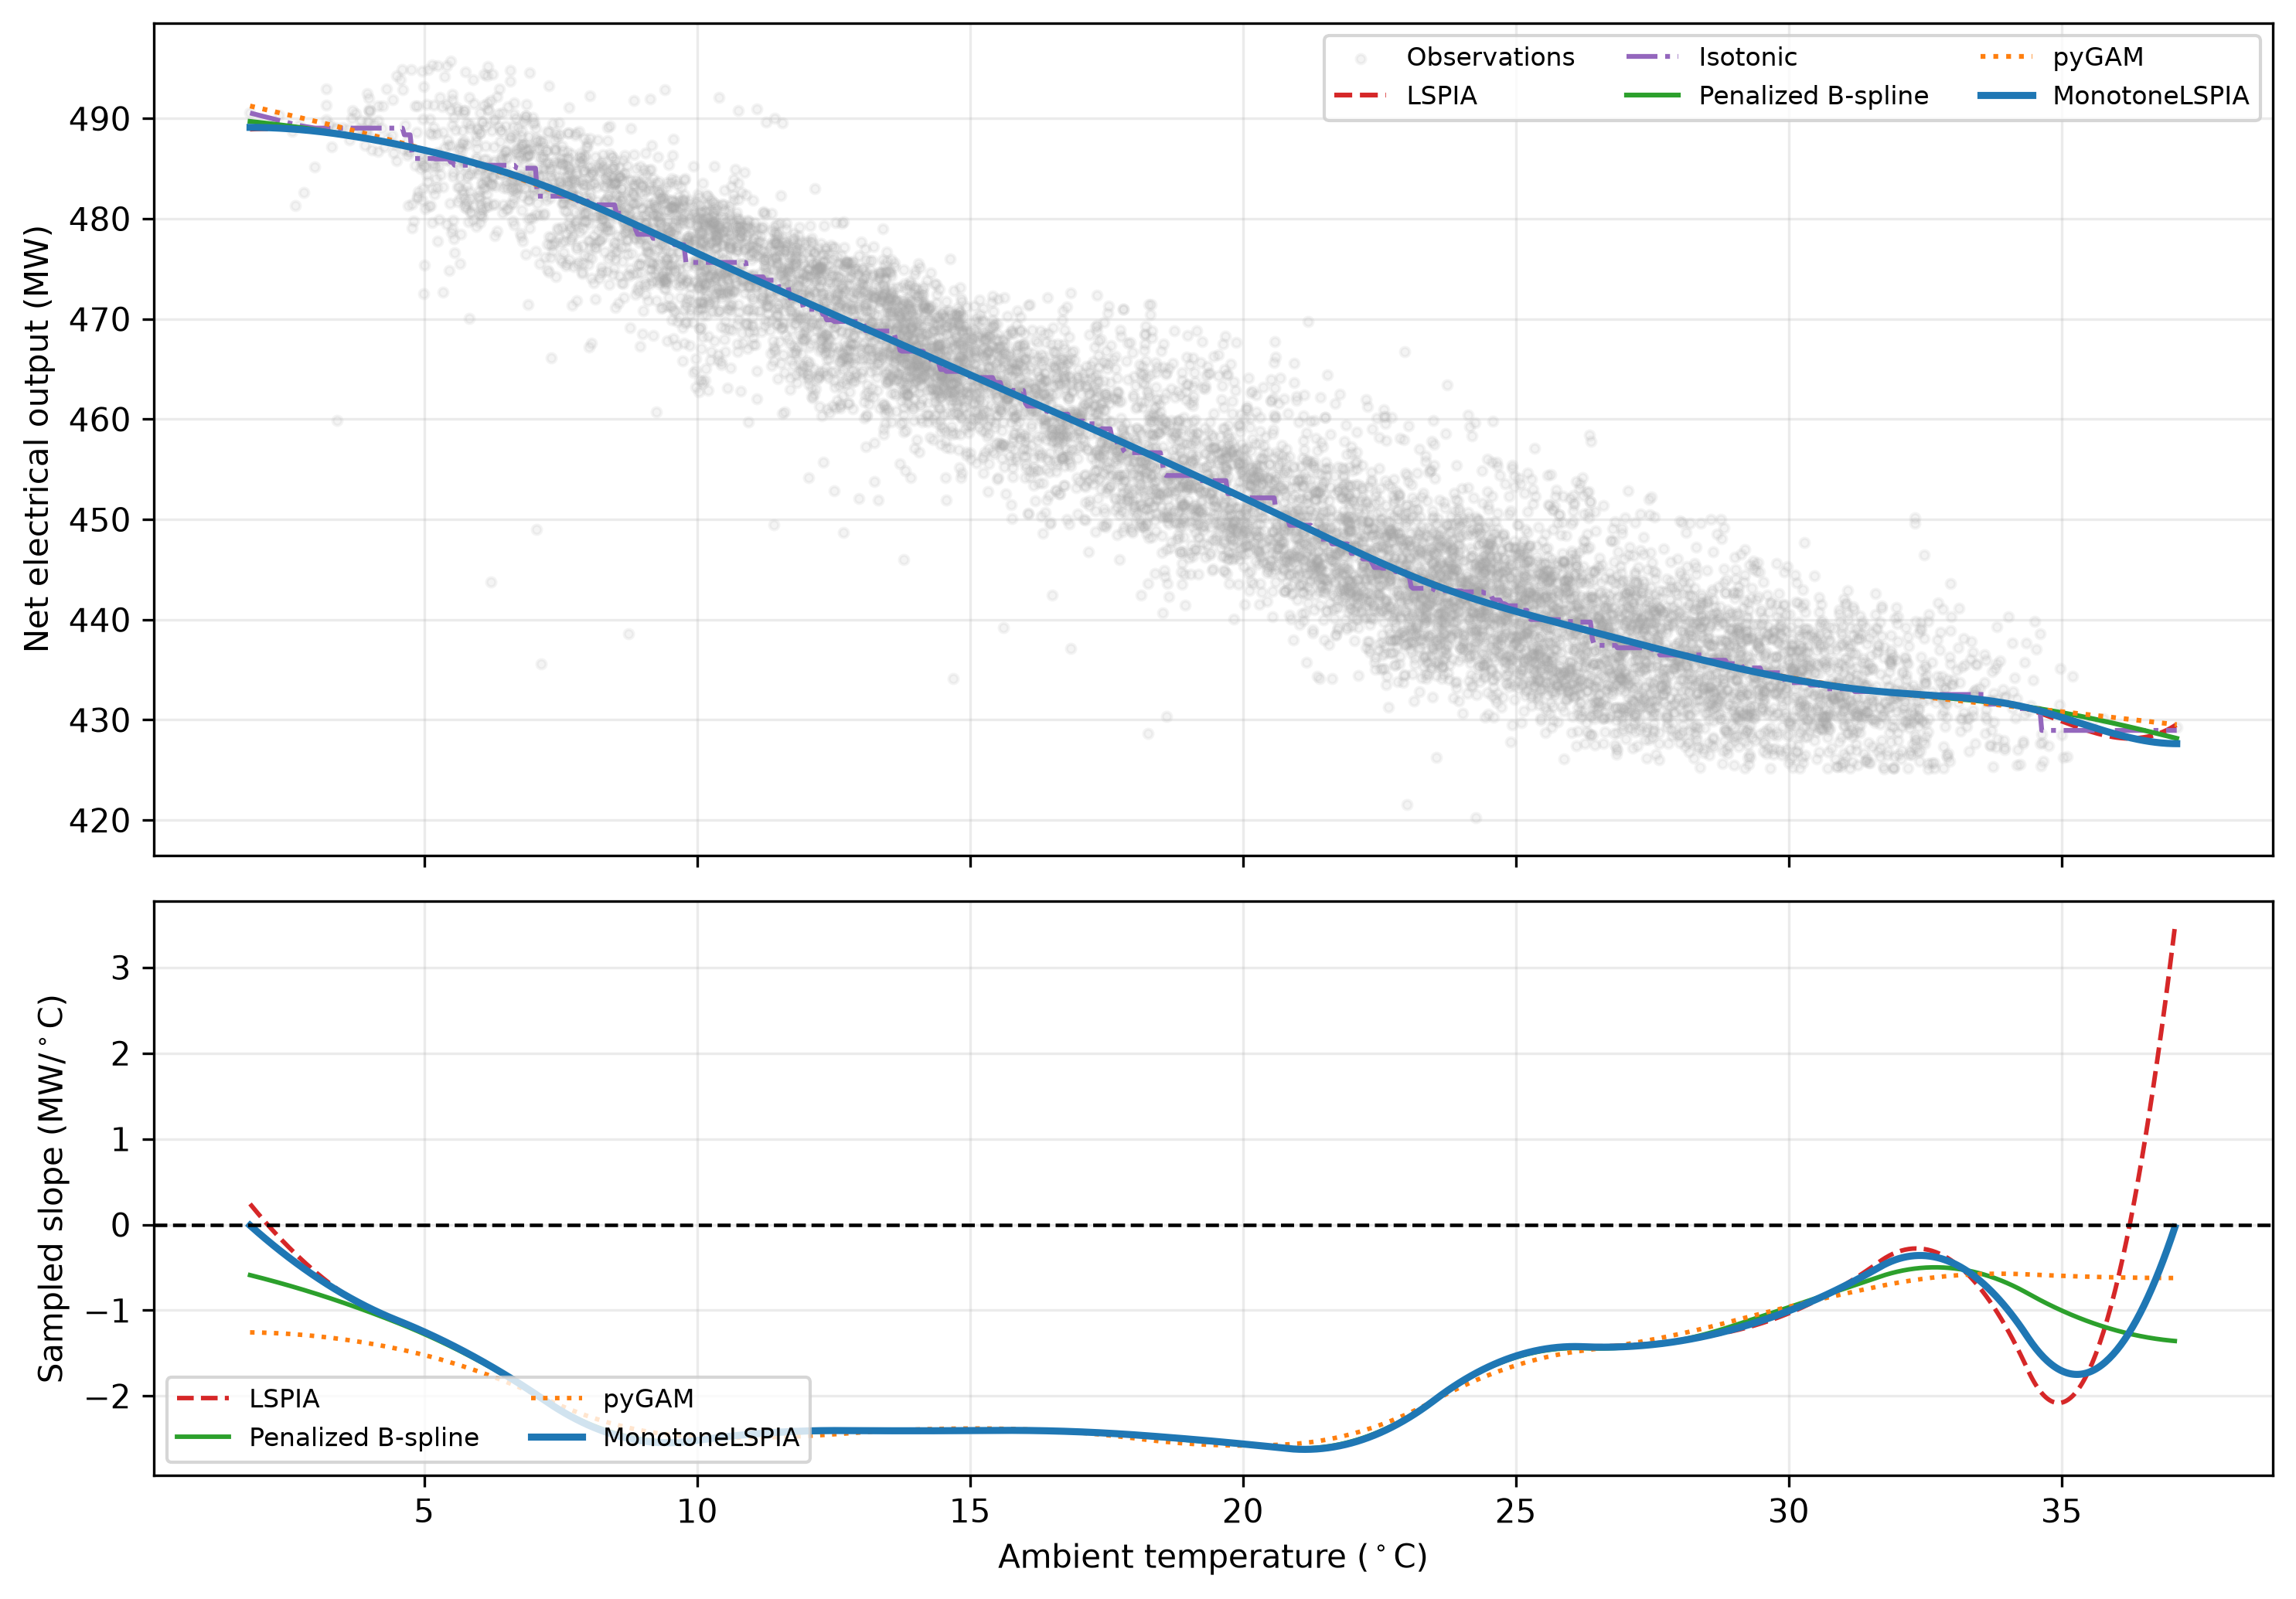
\includegraphics[width=\textwidth]{ccpp_case_study.png}
\caption{Net electrical output versus ambient temperature for all 9568 UCI
power-plant observations. Models were fitted on the deterministic 80\%
training split, and the remaining 20\% produced the results in
Table~\ref{tab:ccpp-results}. The upper panel compares fitted trends for all
five methods. The lower panel shows sampled slopes for the four smooth
methods; positive values indicate violation of the required decreasing
relationship. Isotonic regression is omitted from the slope panel because
its piecewise-linear representation is not differentiable at its
breakpoints. The split seed was 294.}
\label{fig:ccpp}
\end{figure}
\FloatBarrier
